\chapter{Value-Number driven code motion} \label{ch:vdcm}
We implement an iterative bit vector data flow algorithm for PRE. We initially
implemented the flow equations from the Lazy Code Motion paper. This set
included a total of 13 bit vectors for each basic block - 2 for block local
properties ANTLOC and TRANSP, and 11 for global properties. These equations,
           however, could only be applied to single instruction basic blocks.
           We therefore, derive a new set of equations which are motived by a
           later work of the same authors of LCM
           paper\cite{Knoop:1994:OCM:183432.183443}. This set of equations
           apply to maximal basic blocks and entails a total of 19 bit vectors
           for each basic block in our current implementation - 3 for block
           local properties ANTLOC, TRANSP, XCOMP and 16 for global properties.
           We include the equations in appendix A. In appendix B, we
           provide our generalized data flow framework, and show how each PRE
           equation maps to the framework. We call the algorithm value-number driven
           because each slot in each of the bit vectors is reserved for a
           particular value number rather than a particular expression. Also,
           we make the observation that a large number of expressions in the
           program only occur once, and are not useful for PRE. Hence to
           further optimize for space and time, we only give bit vector slots to
           value numbers which have more than one expression linked to them.

% This section on computation of localized sets can be moved to the appendix / not included in 1st report
% Also, check if the definition of XCOMP in terms of TRANSP and EVAL holds.
\section{Computation of localized sets}
For each basic block there are 3 bit vectors dedicated to the block-specific
properties, namely \texttt{Transp}, \texttt{Antloc} and \texttt{Xcomp}. As mentioned before, a bit vector
is a boolean array of value numbers. Each value number is associated with
at-least two expressions from the IR. Let the leader
expression (as defined in the section on value numbering) associated with the
value number $v$ be called $L(v)$. 


\begin{equation}
\begin{array}{l c l}
\texttt{Transp(v,B)} &=& \left\{
                    \begin{array}{l l}
                        false & \quad \text{iff $\exists$ x $\in$ operands of L(v) such that \texttt{Mod(x,B)} = true}\\
                        true & \quad \text{Otherwise}
                    \end{array} \right. \\
\texttt{Antloc(v,B)} &=& \texttt{Eval(v,B)} \cap \texttt{Transp(v,B)} \\
\texttt{Xcomp(v,B)} &=& \texttt{Eval(v,B)} \cap \overline{\texttt{Transp(v,B)}}\\
  &&\\
\text{where}&& \\  
\quad \texttt{Eval(v,B)} &=& \text{\{v $|$ value number v computed in B\}}\\
\quad \texttt{Mod(op,B)} &=& \text{operand op modified in B}\\
\end{array}
\end{equation}

% For the final report we could include an example to show why the definitions of TRANSP, ANTLOC and XCOMP work for value-numbers.
We do not present a formal verification of the definitions of the block local
properties, but in Figure\ref{fig:2}, we motivate these using an example CFG.
\begin{figure}[htbp]
  \begin{center}
    \scalebox{.6}{\begin{tabular}{@{}p{14cm}@{} @{}p{14cm}@{}}
     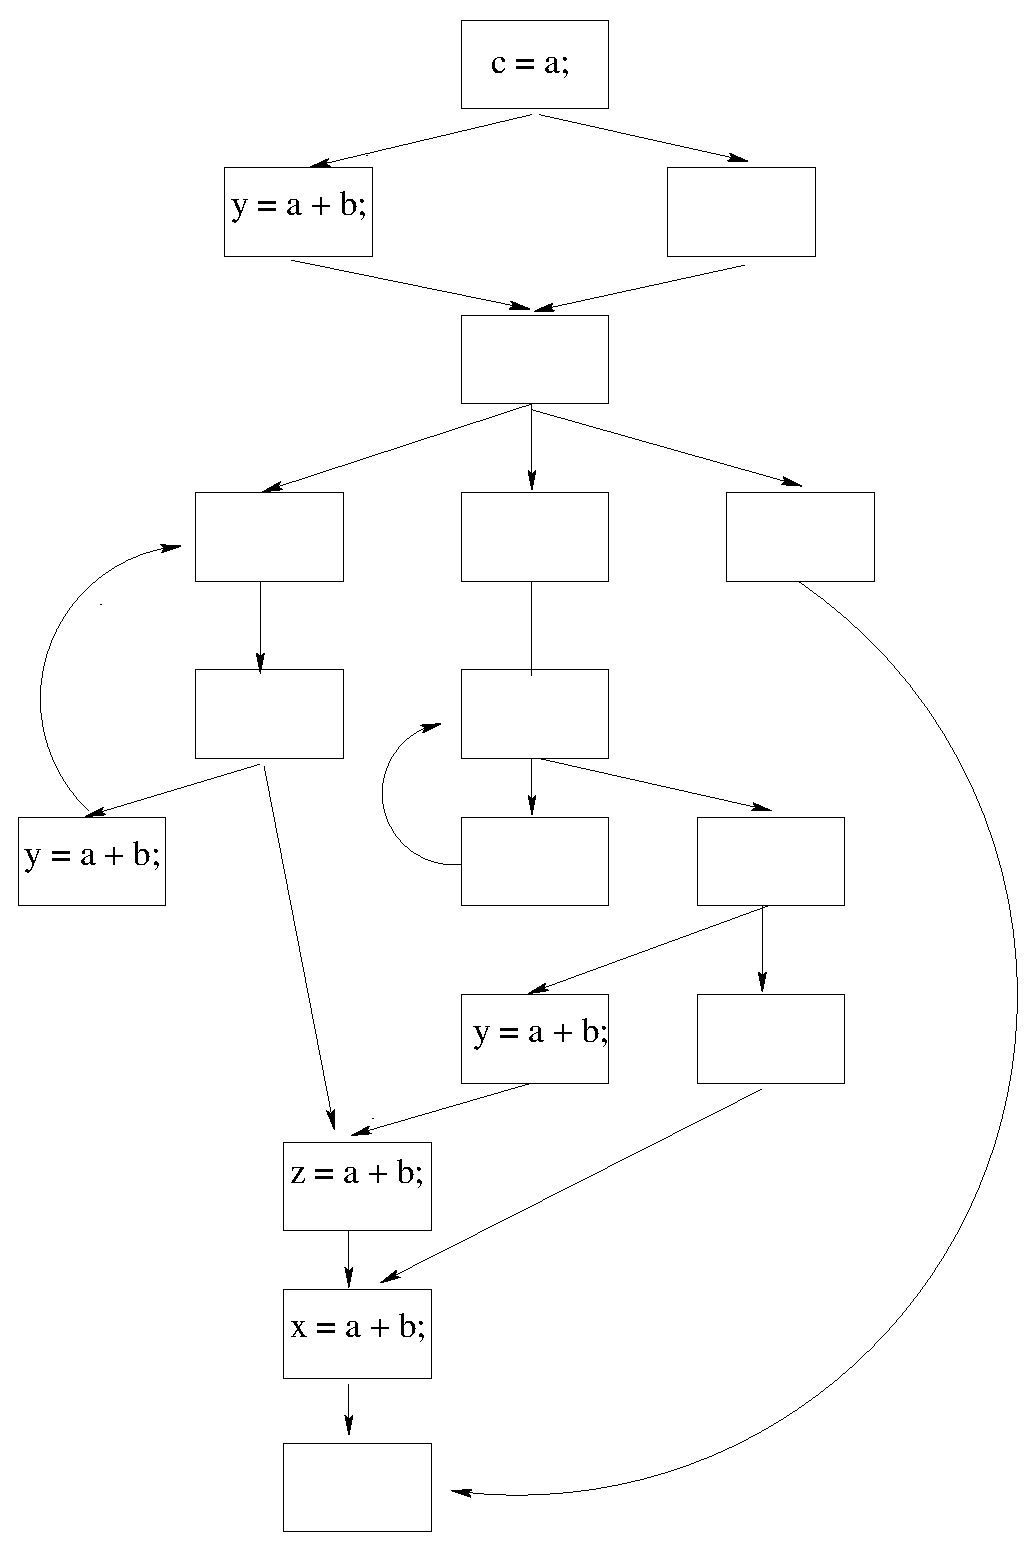
\includegraphics[scale=0.6]{3} & 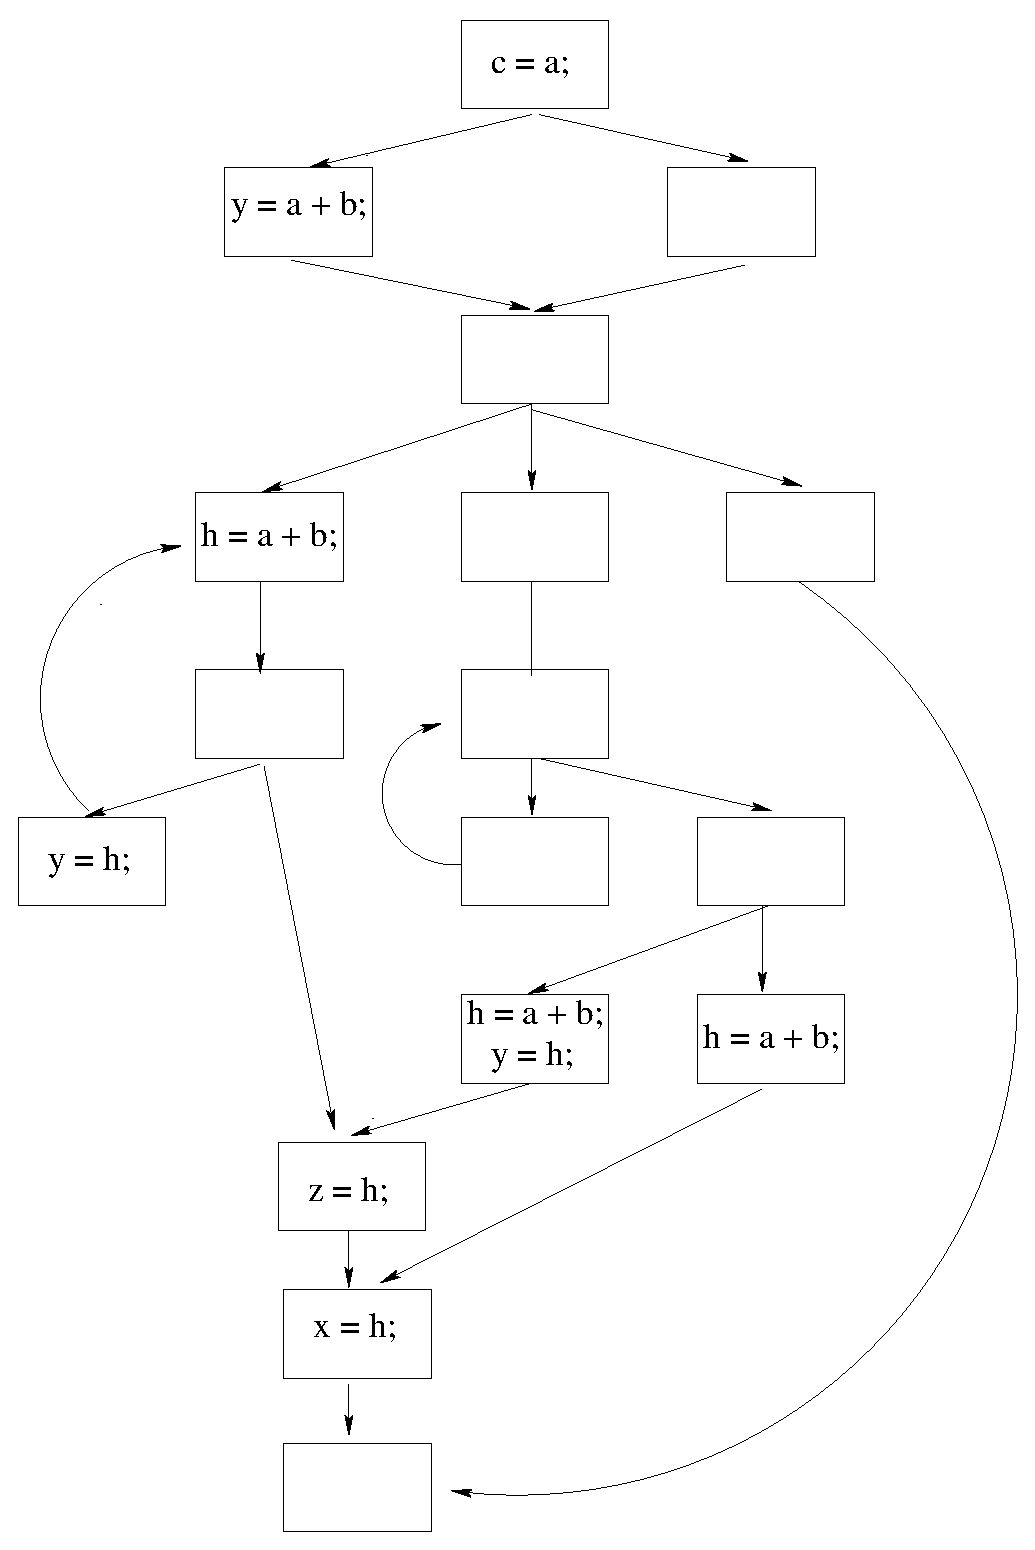
\includegraphics[scale=0.6]{4} \\
      &\\
  \text{The motivating example} &
  \text{Lazy code motion transformation as suggested by our implementation } \\
    \end{tabular}}
  \end{center}
  \caption{\label{fig:2} }
\end{figure}



\section{Local CSE}
For our data flow equations to work correctly, a local CSE pass has to be run
on each basic block. Basically, this path removes the redundancies inside
straight line basic block code and sanitizes it for the iterative bit vector
algorithm. This idea is borrowed from \cite{Knoop:1994:OCM:183432.183443}. We perform this step before calling
our data flow framework. 


\section{Status} 
We summarize accomplished work in this section. We completed the value numbering pass and included some 
optimizations as part of it. We then derived PRE equations for maximal basic block CFG and molded them 
to work with value numbers rather than lexical names. This was followed by construction of a generalized 
data flow framework which could incorporate PRE equations. More specifically, we define a single function 
which can be called with equation specific parameters. We also wrote a pass to perform local CSE on each basic block.
We have tested our implementation of small code segments with good amount of success. We are able to identify 
the placements in the CFG which are computationally optimal as well as lifetime optimal. As an example, we present 
a fairly involved CFG we wrote using goto statements  

\section{Ongoing Work and Future Tasks}
Having identified the INSERT points (where computation should be added) and REPLACE points (from where computation should be removed), 
we are now working on doing the actual IR modifications. Once completed we would begin with testing on fairly large codes for 1) 
correctness and 2) performance improvements. This would be followed by a comparison with the LLVM GVN-PRE pass. Time permitting, 
we would like to provide support for eliminating redundancies where two expressions are lexically different and have different value numbers 
(mentioned in section on PRE)

           
